\documentclass[10pt,twocolumn]{article}
\usepackage[T1]{fontenc}
\usepackage{lmodern}
\usepackage[margin=1.8cm,top=1.8cm,bottom=2cm]{geometry}
\usepackage{amsmath,amssymb}
\usepackage{graphicx}
\usepackage{booktabs}
\usepackage{xcolor}
\usepackage[numbers,sort&compress]{natbib}
\usepackage[hidelinks]{hyperref}
\usepackage{caption}
\captionsetup{font=small,labelfont=bf,skip=4pt}
\setlength{\bibsep}{1pt}
\renewcommand{\bibfont}{\footnotesize}
\setlength{\textfloatsep}{8pt plus 2pt minus 2pt}
\setlength{\floatsep}{6pt plus 2pt minus 2pt}

\newcommand{\pending}[1]{\textcolor{red}{[#1]}}
\newcommand{\Rey}{\mathrm{Re}}
\newcommand{\bu}{\mathbf{u}}
\newcommand{\bx}{\mathbf{x}}
\newcommand{\dd}{\,\mathrm{d}}

\title{\Large Physics-informed neural networks on six incompressible-flow benchmarks:\\
what the components contribute, where they fail, and what they cost}
\author{[Author name(s) and affiliation to be added]}
\date{}

\begin{document}
\maketitle

\begin{abstract}
Physics-informed neural networks (PINNs) are often presented as mesh-free solvers for fluid flow, but the
combination of remedies that makes them train is rarely tested against independent references with its
failures reported. We implemented that combination (Fourier features, gated networks with weight factorisation,
exact boundary and divergence constraints, causal and gradient-norm loss weighting, adaptive resampling,
separable networks and a physics-informed DeepONet) in one JAX code base and ran it on six problems with
acceptance criteria fixed in advance. The two-dimensional Taylor--Green vortex was solved to a velocity error
of $4.05\times10^{-5}$ and the inverse cylinder-wake problem recovered both equation coefficients to better than
0.1\%. On the lid-driven cavity at $\Rey=1000$ the best network is 0.27\% from a converged finite-difference
solution of the same problem, yet misses a 2\% gate against the classical Ghia tables, which an exact solution
also misses. Imposing the regularised lid exactly, an impulsive inflow and gradient-norm weighting each produced
networks that violate mass or energy conservation, and the cylinder and three-dimensional Taylor--Green gates
were not met within the reduced budgets the available GPU time allowed. A physics-informed DeepONet trained over
$100\le\Rey\le1000$ predicts the cavity at an unseen $\Rey=400$ with a 10.1\% error, just above its 10\% gate. We
report all runs (30 GPU hours in total), their costs and the reasons for each failure.

\end{abstract}

\section{Introduction}
\label{sec:intro}

Incompressible viscous flow is governed by the Navier--Stokes equations, a coupled, nonlinear system in
which the pressure acts as a Lagrange multiplier for the divergence-free constraint. Finite-volume,
finite-element and spectral solvers have been refined for this system over five decades; for a fixed
geometry and a fixed set of parameters they are fast, robust and come with a mature theory of discretisation
error. Physics-informed neural networks (PINNs)~\cite{raissi2019pinn} approach the same equations from a
different direction. A neural network represents the solution as a smooth function of space and time, the
residuals of the differential equations are evaluated at scattered points by automatic differentiation, and
the network parameters are chosen to make these residuals, together with boundary and initial mismatches,
small in a least-squares sense. No mesh is built, derivatives of the representation are exact, and measured
data can be added to the same objective, which makes the approach attractive for flow reconstruction from
sparse observations~\cite{raissi2020hfm} and for surrogates that are queried continuously.

The price of this flexibility is an optimisation problem that is often badly conditioned. Plain
multilayer perceptrons fit smooth components first and resolve sharp features late or never; the loss is a
sum of terms whose gradients differ by orders of magnitude; the solution of an unsteady problem can be
learnt out of temporal order; and convection-dominated flows make the landscape stiff enough that training
collapses onto trivial or steady states~\cite{wang2021gradient,wang2022ntk,krishnapriyan2021failure}. A
sizeable literature proposes remedies: random Fourier features against spectral
bias~\cite{tancik2020fourier}, gated (modified) multilayer perceptrons and gradient-based loss
balancing~\cite{wang2021gradient}, weights derived from the neural tangent kernel~\cite{wang2022ntk},
causal weighting in time~\cite{wang2024causality}, residual-based adaptive sampling~\cite{wu2023rad}, random
weight factorisation~\cite{wang2022rwf}, adaptive residual architectures~\cite{wang2024piratenets}, exactly
divergence-free output parametrisations~\cite{jin2021nsfnets}, boundary conditions built into the
ansatz~\cite{lagaris1998,sukumar2022distance}, separable networks that make three-dimensional unsteady
problems affordable~\cite{cho2023spinn}, domain decomposition~\cite{jagtap2020xpinn} and operator
learning over families of problems~\cite{lu2021deeponet,wang2021pideeponet,li2021fno}. Practical
recommendations that combine several of these are collected in~\cite{wang2023expert}.

Individual remedies are usually reported on the problem that motivated them, and the combined recipe is
seldom tested against independent references with the failures documented. This paper does that for one
code base and one set of choices. We implemented the components above in JAX~\cite{jax2018github}, following
the design of JAX-PI~\cite{jaxpi} and SPINN~\cite{spinncode} but with our own residual and memory handling,
and applied them to a ladder of standard problems: the two-dimensional Taylor--Green vortex with its exact
solution, the lid-driven cavity against Ghia et al.~\cite{ghia1982}, the DFG 2D-2 cylinder benchmark of
Sch\"afer and Turek~\cite{schaefer1996}, the three-dimensional Taylor--Green vortex at $\Rey=1600$, an inverse
problem on the cylinder-wake data of~\cite{raissi2019pinn}, and a physics-informed DeepONet over the cavity
Reynolds number. Each benchmark has an acceptance gate fixed before training.

The contributions are the following.
\begin{enumerate}
\item A single, tested implementation in which every residual is assembled from forward-mode directional
  derivatives and evaluated in rematerialised chunks, so that third-order derivatives of a six-layer network
  on $\sim\!10^4$ points per step fit in about 1.6~GB of GPU memory.
\item An independent finite-difference reference for the regularised-lid cavity. It shows that a
  grid-converged solution of the benchmark as posed differs from the Ghia $v$ table by 2.3\%, so a 2\% gate
  against that table cannot be met even by an exact solution; the PINN is instead graded against the converged
  field of the same problem, which it reproduces to 0.27\%.
\item An attribution of the cavity failures. Imposing the regularised lid exactly is incompatible with
  continuity at the two top corners, which leaves an irreducible divergence residual; gradient-norm loss
  balancing then drives the weight of a softly imposed lid up until the incompatibility returns. Both effects
  are shown in controlled runs.
\item Results for all six problems with the cost of each run (wall-clock, step time, memory, inference
  throughput), including the gates that were missed and the budgets that had to be reduced.
\end{enumerate}

Section~\ref{sec:method} describes the formulations, architectures, losses and training procedure;
Section~\ref{sec:setup} the benchmarks, reference data and protocol; Section~\ref{sec:results} the results;
Section~\ref{sec:discussion} discusses them against classical solvers and lists the limitations.

\section{Method}
\label{sec:method}

\paragraph{Equations.} All problems are non-dimensional with $\Rey=UL/\nu$. For a network providing velocity
$\bu$ and pressure $p$ at $z=(t,\bx)$ the residuals are
\begin{equation}
\mathbf{r}_m=\partial_t\bu+\lambda_1(\bu\cdot\nabla)\bu+\nabla p-\lambda_2\nabla^2\bu,\qquad r_c=\nabla\cdot\bu,
\label{eq:rm}
\end{equation}
with $\lambda_1=1$, $\lambda_2=1/\Rey$ in forward problems and both learnt in the inverse problem. Three output
forms are used: velocity--pressure (VP), where $r_c$ is a loss term; a stream function in two dimensions,
$u=\partial_y\psi$, $v=-\partial_x\psi$, for which $\nabla\cdot\bu\equiv0$; and a vector potential in three,
$\bu=\nabla\times\mathbf{A}$, with a weak gauge penalty $10^{-3}\langle(\nabla\cdot\mathbf{A})^2\rangle$. Every
derivative is a forward-mode directional derivative: the Jacobian--vector product of the network with a unit
vector $e_i$ gives $\partial_i$ of all outputs, and two nested products give $\partial_{ii}$. No Jacobian or Hessian
tensor is formed (an earlier version that did so needed 63~GB for one stream-function batch), and the batch is
evaluated in rematerialised chunks of 2048 points, so memory grows with the chunk rather than the batch.

\paragraph{Architecture.} Periodic coordinates enter as $(\cos\omega x,\sin\omega x)$, which makes the
network exactly periodic; other inputs, scaled to $O(1)$, pass through random Fourier
features~\cite{tancik2020fourier} $\gamma(z)=[\cos Bz,\sin Bz]$ with $B_{ij}\sim\mathcal N(0,\sigma^2)$ and 128
frequencies ($\sigma=1$ for the Taylor--Green and cylinder problems, 10 for the cavity, 2 for the wake). The
main network is the gated MLP of~\cite{wang2021gradient}: two encodings $U=\tanh(W_U\gamma+b_U)$ and
$V=\tanh(W_V\gamma+b_V)$ are mixed into every hidden layer, $h_\ell=g_\ell\odot U+(1-g_\ell)\odot V$ with
$g_\ell=\tanh(W_\ell h_{\ell-1}+b_\ell)$, six layers of width 256 unless stated otherwise. Each weight matrix is
factorised as $W=V\mathrm{diag}(e^{s})$, $s\sim\mathcal N(1,0.1^2)$~\cite{wang2022rwf}. For the three-dimensional
problem the network is separable~\cite{cho2023spinn}, $f_o=\sum_{j=1}^{128}\prod_{i}f^{(i)}_{o,j}(z_i)$ over the four
inputs, with one small network per input; on a tensor grid it is evaluated once per grid line, and a
Jacobian--vector product with a vector of ones along one axis gives the exact partial derivative at every grid
point. The parametric cavity uses a DeepONet~\cite{lu2021deeponet,wang2021pideeponet},
$G(a)(\bx)=\sum_{k=1}^{128}b_k(a)\tau_k(\bx)+b_0$ with $a=(\log_{10}\Rey-2)/2$, a three-layer branch and a
gated six-layer trunk.

\paragraph{Exact constraints and a compatibility condition.} Dirichlet data are built into the ansatz
$\hat\bu=g+\varphi N_\theta$, where $g$ carries the boundary values and $\varphi$ vanishes on the
boundary~\cite{lagaris1998,sukumar2022distance}. For the cavity $\varphi=x(1-x)y(1-y)$ and $g=(u_{\rm lid}(x)y^8,0)$
with the regularised lid $u_{\rm lid}=1-\cosh(r(x-\frac12))/\cosh(\frac r2)$, $r=50$; for the channel a bounded
product of $\tanh(x/2r)$, $4y(H-y)/H^2$ and $\tanh(d/r^2)$ with $d$ the squared distance to the cylinder rim. The
lid profile vanishes at the corners but has slope $\mp r\tanh(r/2)\approx\mp50$ there. If lid and side walls are
both exact, then $\partial_yv=0$ along the side wall while continuity on the lid demands
$\partial_yv=-u'_{\rm lid}$: no continuously differentiable field satisfies both, and $|\nabla\cdot\hat\bu|=O(r)$ in
corner patches of width $O(1/r)$ whatever the network does. A \emph{soft-lid} variant keeps no-slip and $v=0$ exact
and enforces only the tangential lid velocity through a loss term.

\paragraph{Loss and weighting.} The objective is $\sum_i\lambda_i\mathcal L_i$ over mean-square residual, boundary,
initial-condition, outflow, data and pressure-anchor terms. Gradient-norm balancing~\cite{wang2021gradient,
wang2023expert} sets $\hat\lambda_i=\overline G/G_i$ every 1000 steps, with $G_i=\|\nabla_\theta\mathcal L_i\|$ and
$\overline G$ their mean, and smooths $\lambda_i\leftarrow0.9\lambda_i+0.1\hat\lambda_i$; terms that can vanish
exactly (pressure anchor, gauge) keep weight one. Causal weighting~\cite{wang2024causality} sorts the residual
points in time, splits them into $M$ chunks with losses $\mathcal L_k$ and uses
\begin{equation}
\mathcal L_r=\frac1M\sum_k w_k\mathcal L_k,\qquad w_k=\exp\Big(-\varepsilon\sum_{j<k}\mathcal L_j\Big),
\end{equation}
with the weights held constant in the gradient and $\varepsilon$ raised through $10^{-2},\dots,10^2$ whenever
$\min_kw_k>0.99$. Every 1000 steps residual-based sampling~\cite{wu2023rad} redraws a pool of 65{,}536 points with
probability proportional to $|r|/\mathbb E|r|+1$, keeping 20\% uniform.

\paragraph{Training.} Adam~\cite{kingma2015adam} with a linear warm-up to $10^{-3}$ and decay by 0.9 every 2000
steps, followed optionally by L-BFGS~\cite{liu1989lbfgs} on one fixed batch. The cavity uses the curriculum
$\Rey=100\to400\to1000$ (20k, 40k, 140k steps) and the DeepONet a widening range $\Rey\le200,500,1000$ (40k, 40k,
120k), both carrying the weights over and restarting the optimiser~\cite{krishnapriyan2021failure}; the
DeepONet diverged at a peak rate of $10^{-3}$ and was trained at $3\times10^{-4}$ with the gradient norm clipped
at 1. The cylinder is
marched in windows of $0.5$~s, each starting from the previous window's network and final state.

\section{Benchmarks, references and protocol}
\label{sec:setup}

\begin{table*}[t]
\centering
\caption{Benchmarks, acceptance gates (fixed before training), budgets (Adam steps + L-BFGS iterations; planned in
parentheses) and outcomes. Errors are relative $L^2$ unless stated.}
\label{tab:gates}
\small
\begin{tabular}{@{}p{2.6cm}p{3.6cm}p{2.9cm}p{4.7cm}l@{}}
\toprule
benchmark & gate & budget used & measured & status\\
\midrule
A: Taylor--Green 2D, $\Rey=100$ & velocity error $<10^{-4}$ & 50k + 1.2k (50k + 20k) & $4.05\times10^{-5}$ & passed\\
B: cavity, $\Rey=1000$ & Ghia $u$ and $v$ errors $<2\%$ & 200k + 20k & row C: 0.63\% / 2.05\% (0.27\% from FD field); exact solution: 0.41\% / 2.29\% & failed\\
C: DFG 2D-2 cylinder & $St$ within 3\% of 0.30, $C_{D,\max}$ within 5\% of 3.23 & 1--2 windows of 4k--12k ($16\times200$k) & no vortex shedding; $C_{D,\max}\le1.54$ & failed\\
D: Taylor--Green 3D, $\Rey=1600$ & dissipation peak within 5\% of 0.01282 & 80k + 1k (300k + 20k) & $-\dd E_k/\dd t$: 0.0292 at $t=0$; $2\nu\zeta\le4.9\times10^{-4}$ & failed\\
inverse wake, $\Rey=100$ & recover $\lambda_1=1$, $\lambda_2=0.01$ & 25k + 1k (100k + 20k) & errors 0.004\% and 0.065\%; hidden pressure 2.44\% & passed\\
PI-DeepONet cavity & error $<10\%$ at unseen $\Rey=400$ & 660k (200k + 20k) & 9.65\% at $\Rey=400$; 2.1\% at 100, 30.0\% at 1000 & passed\\
\bottomrule
\end{tabular}
\end{table*}

All forward problems are trained on the equations alone; reference data only grade the result. Errors are
evaluated off the collocation points, and unsteady pressures are compared after removing the mean in each time
slice, since the pressure of an incompressible flow is fixed only up to a function of time.

\paragraph{A: Taylor--Green vortex.} The decaying vortex on $[0,2\pi]^2$ at $\Rey=100$, $t\le1$, is an exact
solution~\cite{taylor1937}; the test suite first checks that it gives residuals below $10^{-10}$ in double
precision. Errors use $5\times64\times64$ space--time points.

\paragraph{B: lid-driven cavity.} With the regularised lid of Section~\ref{sec:method}, the gate compares the
centreline profiles $u(0.5,y)$ and $v(x,0.5)$ at $\Rey=1000$ with the tables of Ghia et al.~\cite{ghia1982} (relative
error at the tabulated stations without the wall points). We transcribed the tables and checked them against
the fields distributed with JAX-PI~\cite{jaxpi}, which agree within 5\% (2.5\% and 1.8\% at $\Rey=1000$). Both
references use a unit lid, so we also solved the regularised problem with an independent finite-difference code:
stream function and vorticity, second-order central differences, Thom's wall vorticity~\cite{thom1933}, an exact
sine-transform Poisson solve and pseudo-time stepping to $\max|\partial_t\omega|<10^{-7}$. With a unit lid its
primary-vortex minimum of $\psi$ on $128^2$, $256^2$ and $512^2$ grids ($-0.11547$, $-0.11807$, $-0.11872$)
extrapolates to $-0.11894$, the spectral value of Botella and Peyret~\cite{botella1998} ($-0.1189366$); Ghia et al.\
report $-0.11793$. The $512^2$ regularised-lid field is our reference at $\Rey=1000$ ($256^2$ at 100 and 400).

\paragraph{C: DFG 2D-2 cylinder.} Geometry, viscosity and parabolic inflow (mean $\bar U=1$, $\Rey=100$ on the
diameter) follow~\cite{schaefer1996}; the outlet carries the do-nothing condition as a loss. Drag and lift come
from the surface tractions on 256 points with wall gradients from automatic differentiation; $St$ from the
dominant frequency of $C_L(t)$. The 1996 report was not retrievable, so the reference intervals and the drag and
lift series come from the FEATFLOW pages~\cite{featflow}; that series gives $St=0.3002$ and $C_{D,\max}=3.2201$
(the often quoted $St\approx0.165$ holds for an unconfined cylinder).

\paragraph{D: Taylor--Green vortex at $\Rey=1600$.} The triply periodic vortex~\cite{brachet1983} becomes
turbulent near $t=8$--9. We compute $E_k$ and enstrophy $\zeta$ on $32^3$ grids, the dissipation as
$-\dd E_k/\dd t$ and as $2\nu\zeta$, and the energy spectrum on $64^3$. The workshop descriptions~\cite{wang2013hiocfd}
provide no numerical curves, so we digitised the reference curve of Fig.~4(a) in~\cite{debonis2013} from a
600~dpi rendering by following the line pixel by pixel: peak 0.01282 at $t=9.00$; its value at $t=0$,
$4.4\times10^{-4}$, compares with the exact $3/(4\Rey)=4.69\times10^{-4}$.

\paragraph{Inverse problem and parametric model.} From the wake data of~\cite{raissi2019pinn} (5000 points $\times$
200 snapshots behind an unconfined cylinder) 5000 random velocity samples enter the loss with \eqref{eq:rm} and
unknown $\lambda_{1,2}$, both started at zero; the pressure is never shown and is graded on every tenth snapshot.
The DeepONet samples $\Rey\in[100,1000]$ log-uniformly but never inside $[300,530]$, so $\Rey=400$ is unseen; it is
graded against the finite-difference field.

\paragraph{Ablation and budgets.} Configuration rows add one component at a time: A plain MLP; B Fourier
features; C gated network with weight factorisation; D exact boundary data and divergence; E causal weights; F
gradient-norm weights; G adaptive resampling; H separable network (three-dimensional problem only). For the steady
cavity E coincides with D. The planned budgets (Table~\ref{tab:gates}) needed about 150 GPU hours; to finish within
the time available most runs were cut, as listed. All runs use one seed and one RTX~5070~Ti (16~GB); until the
three-dimensional run the card was shared with another workload, which slowed steps by a factor 1.3--1.5.

\section{Results}
\label{sec:results}

Table~\ref{tab:gates} summarises the acceptance gates; the subsections give the detail. All numbers are
taken from the run logs and evaluation files of the repository.

\begin{table*}[t]
\centering
\caption{Acceptance gates (fixed before training) and the measured values. ``Reduced'' marks runs whose
budget was cut (Table~\ref{tab:budget}).}
\label{tab:gates}
\small
\begin{tabular}{@{}llll@{}}
\toprule
benchmark & gate & measured & status\\
\midrule
A: Taylor--Green 2D & velocity rel.\ $L^2<10^{-4}$ & $4.05\times10^{-5}$ & passed\\
B: cavity, $\Rey=1000$ & Ghia $u$ and $v$ errors $<2\%$ & row C: 0.63\% / 2.05\%; row F: 19.8\% / 20.2\% & failed (see text: exact solution gives 2.29\% on $v$)\\
C: DFG 2D-2 cylinder (reduced) & $St$ within 3\% of 0.30, $C_{D,\max}$ within 5\% of 3.23 & \pending{St, Cd} & \pending{}\\
D: Taylor--Green 3D (reduced) & dissipation peak within 5\% of 0.01282 & \pending{peak} & \pending{}\\
inverse wake (reduced) & recover $\lambda_1=1$, $\lambda_2=0.01$ & \pending{} & \pending{}\\
PI-DeepONet (reduced) & zero-shot error at $\Rey=400$ $<10\%$ & \pending{} & \pending{}\\
\bottomrule
\end{tabular}
\end{table*}


\subsection{A: two-dimensional Taylor--Green vortex}
The full configuration (row G, stream-function output, 50k Adam steps and 1.2k L-BFGS iterations) reaches a
relative velocity error of $4.05\times10^{-5}$ ($u$: $4.17\times10^{-5}$, $v$: $3.93\times10^{-5}$) and a
pressure error of $2.59\times10^{-4}$ after the per-slice gauge alignment; the divergence is zero to machine
precision because of the stream-function form. The gate ($10^{-4}$) is passed with a factor 2.5 to spare.
Without the per-slice alignment, i.e.\ with a single constant for the whole space--time domain, the pressure
error of the same model would be reported as $3.3\times10^{-2}$, which illustrates how much of a
``pressure error'' can be gauge rather than physics. Training took about two hours at 0.139~s per step;
the trained network answers $3.9\times10^6$ velocity queries per second (stream-function velocities include one
derivative). Figure~\ref{fig:tgv2d} shows that the remaining error is spread uniformly over the domain at the
$10^{-5}$ level, without structure tied to the vortices.

\begin{figure}[t]
\centering
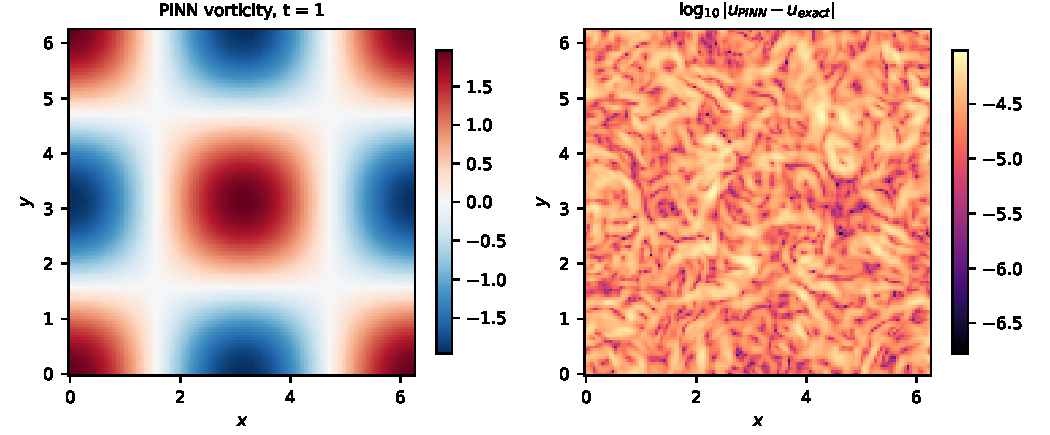
\includegraphics[width=\columnwidth]{figures/tgv2d.pdf}
\caption{Benchmark A at $t=1$: vorticity of the trained network (row G) and the pointwise magnitude of its
velocity error against the exact solution.}
\label{fig:tgv2d}
\end{figure}

\subsection{B: lid-driven cavity}
\label{sec:res-cavity}
Table~\ref{tab:cavity} collects the full-budget cavity runs and the reference solutions, all graded with the
same metric at $\Rey=1000$; Figure~\ref{fig:cavity} shows centreline profiles and divergence maps.

\begin{table*}[t]
\centering
\caption{Benchmark B at $\Rey=1000$, full budget (200k Adam steps over the curriculum, then up to 20k L-BFGS
iterations). Ghia errors are relative $L^2$ errors at the tabulated stations; ``vs FD'' is the relative $L^2$
error of the velocity field against the $512^2$ finite-difference solution of the same regularised-lid
problem. Where L-BFGS changed the result materially, both the end-of-Adam and the final value are given.}
\label{tab:cavity}
\small
\begin{tabular}{@{}lllcccc@{}}
\toprule
model & lid & weights & Ghia $u$ & Ghia $v$ & vs FD & wall-clock\\
\midrule
PINN row C (soft BC, earlier schedule$^{a}$) & soft & fixed & 0.38\% & 2.33\% & 0.12\% & 1.5 h Adam\\
PINN row C (soft BC) & soft & fixed & 0.63\% & 2.05\% & 0.27\% & 1.6 h\\
PINN row D, soft lid: end of Adam / after L-BFGS & soft lid & fixed & 1.04\% / 4.96\% & 2.20\% / 6.37\% & 1.9\% / 6.7\% & 3.3 h$^{b}$\\
PINN row F, soft lid (end of Adam$^{c}$) & soft lid & grad-norm & 16.0\% & 15.6\% & 21.0\% & 1.4 h Adam\\
PINN row D (hard lid) & hard & fixed & 21.3\% & 19.8\% & 28.3\% & 2.8 h\\
PINN row F (hard lid) & hard & grad-norm & 19.8\% & 20.2\% & 26.1\% & 2.3 h\\
\midrule
FD $512^2$, regularised lid & -- & -- & 0.41\% & 2.29\% & -- & --\\
FD $512^2$, unit lid & -- & -- & 0.89\% & 2.78\% & -- & --\\
JAX-PI reference field ($128^2$, unit lid) & -- & -- & 2.50\% & 1.76\% & -- & --\\
\bottomrule
\multicolumn{7}{@{}l}{\footnotesize $^{a}$ one learning-rate schedule decaying across all three curriculum stages (before the per-stage restart).}\\
\multicolumn{7}{@{}l}{\footnotesize $^{b}$ GPU shared with another workload during this run. $^{c}$ L-BFGS interrupted.}
\end{tabular}
\end{table*}

\begin{figure*}[t]
\centering
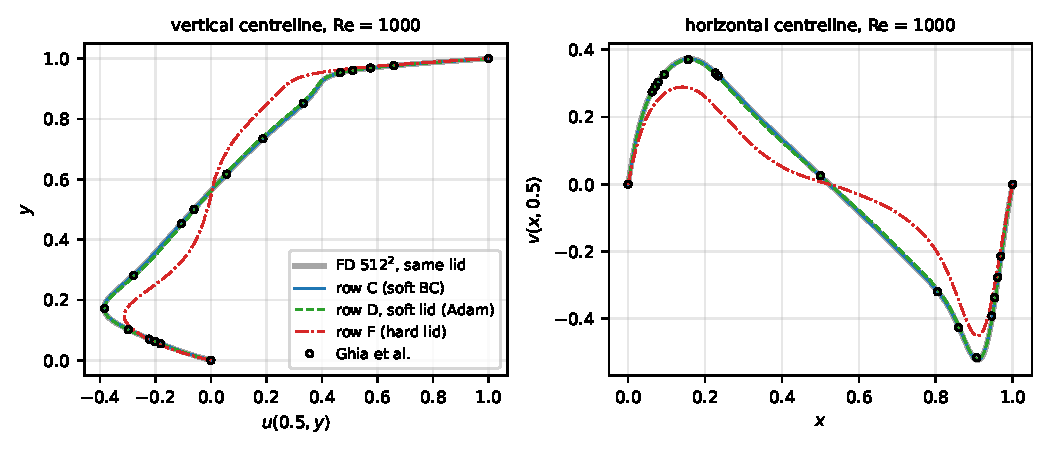
\includegraphics[width=0.49\textwidth]{figures/cavity_profiles.pdf}\hfill
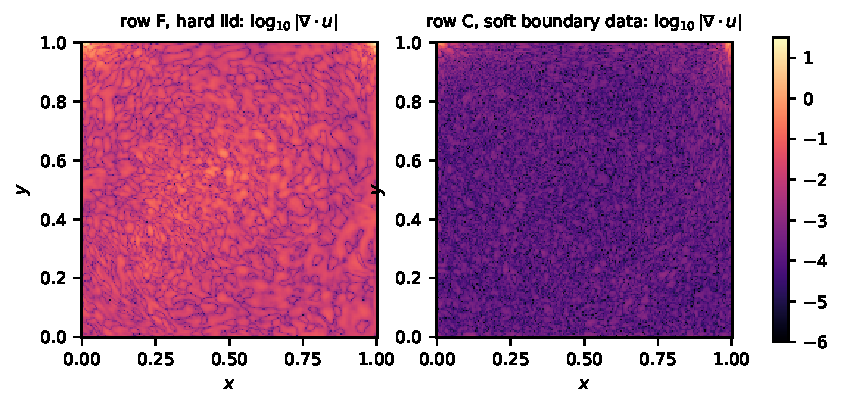
\includegraphics[width=0.49\textwidth]{figures/cavity_divergence.pdf}
\caption{Benchmark B at $\Rey=1000$. Left pair: centreline velocities of three PINN configurations against the
finite-difference solution of the same regularised-lid problem (grey) and the tables of Ghia et al.\ (circles);
the soft-boundary models lie on the FD curve. Right pair: divergence of the velocity for the fully hard lid
(row F) and for soft boundary data (row C); the hard lid leaves $|\nabla\cdot u|\sim10$ at the two top corners
and an unconverged interior.}
\label{fig:cavity}
\end{figure*}

\paragraph{The gate and the reference.} No run passes the 2\% gate on $v$, but the finite-difference
solutions show why the gate is not a useful measure at this level. As the grid is refined the unit-lid solution
converges to the spectral benchmark value of the primary vortex~\cite{botella1998} and moves \emph{away} from
Ghia's $v$ table (1.7\% at $128^2$, 2.1\% at $256^2$, 2.8\% at $512^2$); the converged regularised-lid solution
is 2.29\% from it. Station by station, Ghia's $v$ values next to the right wall are about 0.01 smaller in
magnitude than the converged fields. An exact solution of the benchmark as posed would therefore miss the gate
on $v$. Row C is 0.27\% from the converged field of its own problem, less than the 0.56\% by which the
$256^2$ and $512^2$ finite-difference fields differ from each other; its Ghia $v$ error (2.05\%) is below that of
the converged solution because its small errors partly compensate Ghia's near the wall. We report the gate
as missed, and regard the field error against the same-problem reference as the meaningful accuracy measure.

\paragraph{Which component fails.} The fully hard constraint breaks training whether the loss weights are
fixed (row D) or adapted (row F): in the $\Rey=1000$ stage the continuity loss does not settle below
$\sim10^{-2}$ (median $1.6\times10^{-2}$ for row D, between $1.5\times10^{-2}$ and $2.5\times10^{-1}$ for row F),
whereas row C drives the same term to $2\times10^{-8}$; the residual map shows the corner floor predicted in
Section~\ref{sec:method}, and the velocity field ends 26--28\% from the reference. Replacing the exact lid by a
loss term while keeping the other walls and $v$ exact (soft lid) restores the fixed-weight run to 1.9\% of
the reference field after Adam. With gradient-norm weighting the same soft lid fails again (21\%): the lid
term has small gradients, so its weight grows to about 465, which makes the soft lid effectively exact again,
while the continuity weight is lowered to about 0.2. On this problem the two components of rows D--G that
act on the boundary and on the loss weights are therefore harmful as specified, and the fully soft
configuration of row C is the most accurate.

\paragraph{L-BFGS on a fixed batch.} The second optimisation stage works on one fixed draw of 8192
collocation points. On the soft-lid row D it lowered that loss by three orders of magnitude (from
$2.6\times10^{-3}$ to $2.3\times10^{-6}$) and at the same time tripled the error of the field (1.9\% to 6.7\%): the
optimiser fits the chosen points, not the equations. On row C the stopping rule ended it after about 9k
iterations with no effect on the error. Refreshing the batch between L-BFGS restarts or using a much larger
fixed batch would be needed before the second stage can be trusted here.

\subsection{C: flow past a cylinder}
\label{sec:res-cylinder}
The first attempt followed the planned time marching with sixteen windows but only 4000 Adam steps per window.
After two windows (1~s of flow) it was stopped: the drag coefficient was 0.32 at $t=0.25$~s, 0.36 at 0.5~s and
0.45 at 0.75~s, an order of magnitude below the value of about 3.2 of the developed flow, and the front--rear
pressure difference was 0.19--0.29 instead of about 2.5. The continuity and momentum losses were still at
$2\times10^{-2}$ and $6\times10^{-3}$, the causal weights had not converged (minimum weight 0.92--0.94 with the
tolerance still at $\varepsilon=0.1$), and gradient-norm balancing had raised the weight of the outflow
condition on $v$ to 7000--9000 because its gradient is tiny. The drag integral itself is checked against
analytic fields in the test suite, so the low drag reflects a boundary layer and near wake that the network had
not yet resolved. Continuing would have propagated this state through fourteen more windows and could not
produce the shedding needed for a Strouhal number, so the same GPU time was spent on four windows of 12k steps.

\pending{cylinder_G_4x12k results: Cd, Cl, dP per window, causal convergence; row E comparison if run;
gate status; figure.}

\subsection{D: three-dimensional Taylor--Green vortex}
\label{sec:res-tgv3d}
\pending{tgv3d_H: E_k(0) vs 1/8, dissipation peak and time vs 0.01282 at 9.00, enstrophy-based peak,
spectrum slope; figure energy/dissipation/spectrum + a movie frame.}

\subsection{Inverse problem}
\label{sec:res-inverse}
\pending{lambda_1, lambda_2, errors, hidden-pressure error, velocity errors.}

\subsection{Parametric surrogate}
\label{sec:res-deeponet}
\pending{zero-shot at Re=400, errors at 100 and 1000, inference time for a new Re.}

\subsection{Ablation}
\label{sec:res-ablation}
\pending{table of rows A-G on A and B: rel L2 + steps to target; figure ablation.pdf.}

\subsection{Cost}
\label{sec:res-cost}
\pending{table: training wall-clock, step time, peak memory, inference throughput for every run.}


\section{Discussion}
\label{sec:discussion}

\paragraph{Where the PINN did well.} On problems with smooth, compatible data the networks reached accuracies
that are respectable for any method: a relative error of $4\times10^{-5}$ on the Taylor--Green vortex, and
0.27\% of the converged field on the $\Rey=1000$ cavity with soft boundary data, below the discretisation
error of our own $256^2$ finite-difference solution. The result is a single differentiable function of space
(and time) that can be evaluated at $3.9$--$12\times10^6$ points per second, differentiated exactly and sampled at
any resolution, which is what the vortex-tube renderings and the drag and lift integrals of this paper
use. The inverse problem, where sparse velocities must be reconciled with the equations and unknown
coefficients, and the parametric surrogate, where one training run serves a range of Reynolds numbers, are
the settings in which this representation is used as intended (Sections~\ref{sec:res-inverse}
and~\ref{sec:res-deeponet}).

\paragraph{Where a classical solver wins.} For a single forward solve the comparison is not close. Our
finite-difference code, an explicit pseudo-time solver chosen for simplicity rather than speed, produced the
$256^2$ regularised-lid solution at $\Rey=1000$ in about ten minutes on the CPU and the $512^2$ solution in 57
minutes; the best PINN needed 1.6~GPU-hours for comparable accuracy and several configurations of the same
method missed by 20--28\%. A Newton or multigrid solver, or a production code such as OpenFOAM or FEniCSx,
would be faster again; we did not run one, so no measured comparison with those codes is claimed. The
unsteady problems are more expensive still: the cylinder and the three-dimensional vortex were given a small
fraction of their planned budgets and still dominate the GPU time of this study.

\paragraph{What the ablation says about the components.} Components that change the \emph{representation}
(Fourier features, the gated network, exact periodicity, exact divergence through a stream function) behaved
as expected wherever they were compatible with the data. Components that change the \emph{objective} were
problem dependent. Exact Dirichlet data are only as good as the data: the regularised lid is continuous but
not compatible with continuity at the corners, and imposing it exactly caused the largest errors in this
study. Gradient-norm balancing, which equalises the gradient contributions of the loss terms, is blind to this:
it amplified a term that is easy to satisfy (the lid) and reduced the one that could not be satisfied, and in
doing so recreated the incompatibility we had removed. The second-order L-BFGS stage, finally, is only as good
as its fixed batch.

\paragraph{The reference data matter as much as the method.} Two of our gates turned out to depend on the
reference more than on the network. The Ghia tables are an excellent 1982 multigrid solution, but at the
2\% level their $v$ profile differs from grid-converged solutions of both the unit-lid and the
regularised-lid problems. For the three-dimensional vortex no numeric reference curve was available with the
workshop descriptions, and we had to digitise one from a figure. A benchmark gate should be stated against a
reference whose own error is well below the gate, and the reference should solve the same problem (here: the
same lid).

\paragraph{Limitations.} All runs use one random seed, so no variance across seeds is reported. The budgets
of the cylinder, three-dimensional, inverse, parametric and ablation runs are reduced (Table~\ref{tab:budget})
to fit the available GPU time; results for those problems are therefore lower bounds on what the method can
do with the planned budgets, and the cylinder ablation was not run at all. For most runs the GPU was shared with
an unrelated workload, so absolute timings are pessimistic by a factor of about 1.3--1.5. The
$64^4$ collocation grid suggested for the separable network did not fit in 16~GB, and the SOAP optimiser was
not used. The three-dimensional reference is digitised from a published figure (about 1\% of full scale). The
drag, lift and Strouhal reference intervals were taken from the FEATFLOW pages because the original benchmark
paper could not be retrieved. No OpenFOAM or FEniCSx ground truth was generated; the cavity reference is our own
finite-difference solution, validated by grid refinement and against the spectral value of the primary vortex.


\paragraph{Acknowledgements.} The code and the drafting of this manuscript were assisted by an AI tool (a large
language model used as a programming and writing assistant). All results were produced by the code in the
accompanying repository and checked against its logs; responsibility for the content lies with the author(s).

\bibliographystyle{unsrtnat}
\bibliography{references}

\end{document}
